Hiperparametry najlepszej architektury (ResNet50) dobrano biblioteką \textbf{Optuna}
(\texttt{src/tune.py}, notatnik \texttt{04\_tuning\_optuna.ipynb}). Jest to optymalizacja
bayesowska, a nie przeszukiwanie siatki ani losowe. Próbnik TPE (Tree-structured Parzen
Estimator) dzieli dotychczasowe próby na lepsze i gorsze, modeluje rozkład hiperparametrów
w obu grupach i proponuje konfiguracje, dla których stosunek tych rozkładów jest największy.
Słabe próby przerywa MedianPruner: po każdym foldzie porównuje średni wynik próby z medianą
wcześniejszych prób na tym samym etapie (idea Successive Halving z wykładu).

Przestrzeń poszukiwań: LR głowicy $10^{-4}$--$3\cdot10^{-3}$ (skala logarytmiczna), weight decay
$10^{-6}$--$10^{-2}$ (log.), dropout 0--0,5, batch size \{16, 32, 64\}, liczba odmrożonych
bloków szkieletu 1--\nBlocks{}. Funkcja celu to średnie macro-F1 na foldach walidacyjnych 0--2
(10 epok na próbę). Zbiór testowy nie był używany. Badanie liczy \nTrials{} prób
(\nTrialsComplete{} zakończonych, \nTrialsPruned{} przyciętych). Dodatkowo jedna próba została
przerwana przez wyłączenie komputera. Optuna zapisuje próby w bazie SQLite, więc strojenie wznowiono
i dokończono do \nTrials{} prób.

Najlepsza konfiguracja: LR $\optLr$, weight decay $\optWd$, dropout \optDropout{}, batch size
\optBatch{}, \optUnfreeze{} odmrożone bloki. Najważniejszym hiperparametrem okazał się LR
(ważność fANOVA \impLr{}), potem dropout (\impDropout{}) i weight decay (\impWd{}).

\begin{figure}[H]
\centering
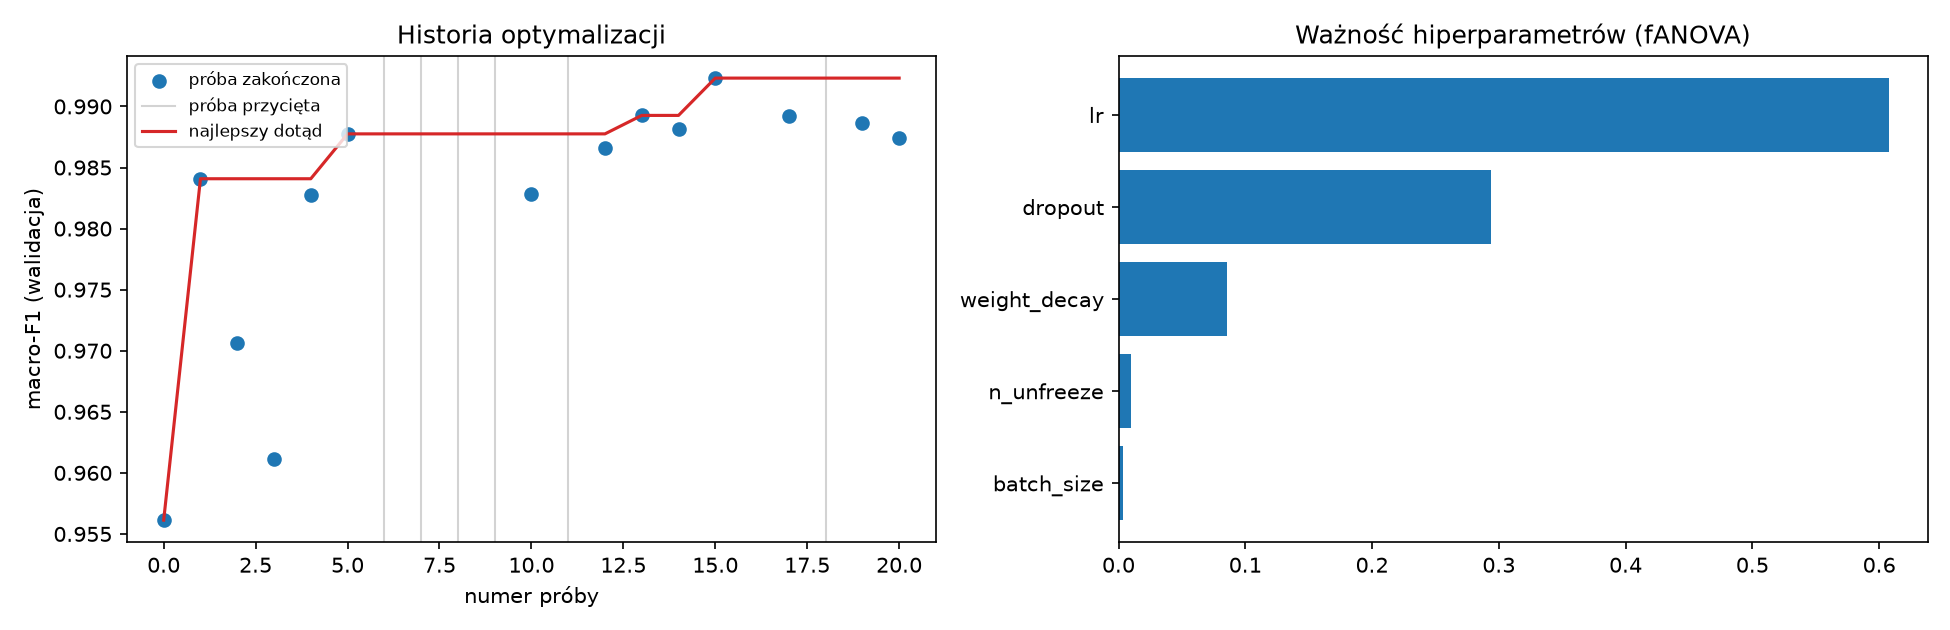
\includegraphics[width=\linewidth]{optuna.png}
\caption{Historia optymalizacji (szare linie -- próby przycięte) i ważność hiperparametrów.}
\label{fig:optuna}
\end{figure}

\paragraph{Ryzyko przeoptymalizowania na walidacji.} Najlepsza próba osiągnęła na walidacji
macro-F1 \optBest{}, ale ta liczba jest zawyżona. Wybieramy maksimum z wielu prób liczonych na
tych samych foldach, więc część przewagi to przypadek (wykład~4). W pełnej 5-krotnej walidacji
parametry po strojeniu dały \cvFResTuned{} $\pm$ \cvFsdResTuned{} wobec \cvFRes{} $\pm$ \cvFsdRes{}
dla parametrów domyślnych. Poprawa jest mniejsza niż odchylenie między foldami, a foldy 0--2
służyły do strojenia. Poprawną metodą byłaby zagnieżdżona walidacja krzyżowa, jednak jest
ok.~5 razy droższa obliczeniowo. Ostatecznym sprawdzianem był test: po strojeniu macro-F1 na
\texttt{test\_dedup} wzrosło z \fDedupRes{} do \fDedupResTuned{}, ale przedziały ufności
się pokrywają.
